%%%%%%%%%%%%%%%%%%%%%%%%%%%%%%%%%%%%%%%%%
% Contract
% LaTeX Template
% Version 1.0 (December 8 2014)
%
% This template has been downloaded from:
% http://www.LaTeXTemplates.com
%
% Original author:
% Brandon Fryslie
% With extensive modifications by:
% Vel (vel@latextemplates.com)
%
% License:
% CC BY-NC-SA 3.0 (http://creativecommons.org/licenses/by-nc-sa/3.0/)
%
% Note:
% If you are using Apple OS X, go into structure.tex and uncomment the font
% specifications for OS X and comment out the default specifications - this will
% drastically increase how good the document looks. You will now need to
% compile with XeLaTeX.
%
%%%%%%%%%%%%%%%%%%%%%%%%%%%%%%%%%%%%%%%%%

\documentclass[a4paper,12pt]{article} % The default font size is 12pt on A4 paper, change to 'usletter' for US Letter paper and adjust margins in structure.tex

\usepackage{url}
\usepackage{multirow}
\usepackage{hyperref}
\usepackage{graphicx}
\usepackage{color}
\usepackage{listings}
\usepackage{setspace}
\definecolor{Code}{rgb}{0,0,0}
\definecolor{Decorators}{rgb}{0.5,0.5,0.5}
%\definecolor{Numbers}{rgb}{0.5,0,0}
\definecolor{MatchingBrackets}{rgb}{0.25,0.5,0.5}
\definecolor{Keywords}{rgb}{0,0,1}
\definecolor{self}{rgb}{0,0,0}
\definecolor{Strings}{rgb}{0,0.63,0}
\definecolor{Comments}{rgb}{0,0.63,1}
\definecolor{Backquotes}{rgb}{0,0,0}
\definecolor{Classname}{rgb}{0,0,0}
\definecolor{FunctionName}{rgb}{0,0,0}
\definecolor{Operators}{rgb}{0,0,0}
\definecolor{Background}{rgb}{0.98,0.98,0.98}
\lstdefinelanguage{Python}{
%numbers=left,
%numberstyle=\footnotesize,
%numbersep=1em,
xleftmargin=1em,
framextopmargin=2em,
framexbottommargin=2em,
showspaces=false,
showtabs=false,
showstringspaces=false,
frame=l,
tabsize=4,
% Basic
basicstyle=\ttfamily\small\setstretch{1},
backgroundcolor=\color{Background},
% Comments
commentstyle=\color{Comments}\slshape,
% Strings
stringstyle=\color{Strings},
morecomment=[s][\color{Strings}]{"""}{"""},
morecomment=[s][\color{Strings}]{'''}{'''},
% keywords
morekeywords={import,from,class,def,for,while,if,is,in,elif,else,not,and,or,print,break,continue,return,True,False,None,access,as,,del,except,exec,finally,global,import,lambda,pass,print,raise,try,assert},
keywordstyle={\color{Keywords}\bfseries},
% additional keywords
morekeywords={[2]@invariant,pylab,numpy,np,scipy},
keywordstyle={[2]\color{Decorators}\slshape},
emph={self},
emphstyle={\color{self}\slshape},
%
}
\hypersetup{
    colorlinks=true,
    linkcolor=blue,
    filecolor=magenta,      
    urlcolor=blue,
    citecolor=blue
}

%%%%%%%%%%%%%%%%%%%%%%%%%%%%%%%%%%%%%%%%%
% Contract
% Structural Definitions File
% Version 1.0 (December 8 2014)
%
% Created by:
% Vel (vel@latextemplates.com)
% 
% This file has been downloaded from:
% http://www.LaTeXTemplates.com
%
% License:
% CC BY-NC-SA 3.0 (http://creativecommons.org/licenses/by-nc-sa/3.0/)
%
%%%%%%%%%%%%%%%%%%%%%%%%%%%%%%%%%%%%%%%%%

%----------------------------------------------------------------------------------------
%	PARAGRAPH SPACING SPECIFICATIONS
%----------------------------------------------------------------------------------------

\setlength{\parindent}{0mm} % Don't indent paragraphs

\setlength{\parskip}{2.5mm} % Whitespace between paragraphs

%----------------------------------------------------------------------------------------
%	PAGE LAYOUT SPECIFICATIONS
%----------------------------------------------------------------------------------------

\usepackage{geometry} % Required to modify the page layout

\setlength{\textwidth}{16cm} % Width of the text on the page
\setlength{\textheight}{24.5cm} % Height of the text on the page

\setlength{\oddsidemargin}{0cm} % Width of the margin - negative to move text left, positive to move it right

% Uncomment for offset margins if the 'twoside' document class option is used
%\setlength{\evensidemargin}{-0.75cm} 
%\setlength{\oddsidemargin}{0.75cm}

\setlength{\topmargin}{-1.25cm} % Reduce the top margin

%----------------------------------------------------------------------------------------
%	FONT SPECIFICATIONS
%----------------------------------------------------------------------------------------

% If you are running Apple OS X, uncomment the next 4 lines and comment/delete the block below, you will now need to compile with XeLaTeX but your document will look much better

%\usepackage[cm-default]{fontspec}
%\usepackage{xunicode}

%\setsansfont[Mapping=tex-text,Scale=1.1]{Gill Sans}
%\setmainfont[Mapping=tex-text,Scale=1.0]{Hoefler Text}

%-------------------------------------------

\usepackage[utf8]{inputenc} % Required for including letters with accents
\usepackage[T1]{fontenc} % Use 8-bit encoding that has 256 glyphs

\usepackage{avant} % Use the Avantgarde font for headings
\usepackage{mathptmx} % Use the Adobe Times Roman as the default text font together with math symbols from the Sym­bol, Chancery and Com­puter Modern fonts

%----------------------------------------------------------------------------------------
%	SECTION TITLE SPECIFICATIONS
%----------------------------------------------------------------------------------------

\usepackage{titlesec} % Required for modifying section titles

\titleformat{\section} % Customize the \section{} section title
{\sffamily\large\bfseries} % Title font customizations
{\thesection} % Section number
{16pt} % Whitespace between the number and title
{\large} % Title font size
\titlespacing*{\section}{0mm}{7mm}{0mm} % Left, top and bottom spacing around the title

\titleformat{\subsection} % Customize the \subsection{} section title
{\sffamily\normalsize\bfseries} % Title font customizations
{\thesubsection} % Subsection number
{16pt} % Whitespace between the number and title
{\normalsize} % Title font size
\titlespacing*{\subsection}{0mm}{5mm}{0mm} % Left, top and bottom spacing around the title % Input the structure.tex file which specifies the document layout and style

%----------------------------------------------------------------------------------------
%	DYNAMIC CONTRACT INFORMATION
%----------------------------------------------------------------------------------------

% Your name and company name
\newcommand{\YourName}{[Your name]}
\newcommand{\CompanyName}{[Company name]}

% Your address
\newcommand{\AddressLineOne}{[Address]}
\newcommand{\AddressLineTwo}{[Address]}

% Your email address
\newcommand{\YourEmail}{[Your email]}

% The client's name
\newcommand{\ClientName}{[Client name]}

% The delivery date for specifications and completion date for the project
\newcommand{\DeliveryDate}{[date]}
\newcommand{\CompletionDate}{[date]}

% The hourly rate
\newcommand{\HourlyRate}{\$25}

% Payee's information
\newcommand{\PayeeName}{[Payee Name]}
\newcommand{\PaymentAddressLineOne}{[Adress]}
\newcommand{\PaymentAddressLineTwo}{[Adress]}
\newcommand{\PaymentAddressLineThree}{[Adress]}

%----------------------------------------------------------------------------------------

\begin{document}

%----------------------------------------------------------------------------------------
%	TITLE PAGE
%----------------------------------------------------------------------------------------

\begin{titlepage}

\vspace*{\fill} % Add whitespace above to center the title page content

\begin{center}

{\LARGE A fake news detector}
\vspace{1.5cm}

{\large Capstone Project\\ Udacity Machine
  Learning Engineer Nanodegree}\\ [1.5cm]

Submitted: \today

\end{center}

Author: Stefano Casasso\\

\vspace*{\fill} % Add whitespace below to center the title page content

\end{titlepage}

%----------------------------------------------------------------------------------------
%	DEFINITION SECTION
%----------------------------------------------------------------------------------------

\section{Definition}


\subsection{Project Overview}
\label{sec:overview}
As opposed to \textit{real news}, which is based on true facts
and has the goal of informing the audience,
\textit{fake news} can be defined as ``a made-up story with an
intention to deceive'' \cite{NYT}.
Fake news is probably as old
as real news, but it has become a major problem with the coming of the
web which made it extremely easy and fast to circulate contents
among a potentially very large number of people. In particular, with
the success of social networks in the last decade, fake news are
spread around like a virus by people, usually with limited education and
background, who share them in their public profiles.

The aim of this project is to build an algorithm to detect and flag fake news,
based only on the text of the news. This is a \textit{binary classification problem} which
is studied using supervised machine learning (ML) techniques.
In order to successfully apply these techniques,
a sizeable ``labelled'' dataset is needed, preferably with a good balance
between the different classes in output (fake, real). \\
A dataset for fake news is already
publicly available on the popular data science platform
\href{https://www.kaggle.com}{Kaggle} \cite{KaggleDataset}. \\
This dataset is built by crawling the news from 244 websites which are
tagged as not reliable sources by the
\href{https://github.com/selfagency/bs-detector}{BS Detector} project.
BS Detector ultimately uses a manually compiled list taken
from the \href{http://www.opensources.co/}{OpenSources} platform.
As does Kaggle, we consider this an authority in the domain of fake
news and we assume that these data are purely fake news. \\
For the ``real'' news, we use the freely downloadable dataset from
\href{https://webhose.io/datasets}{webhose.io}, under ``English news
articles''.
Both the fake and real news come from November 2016.


\subsection{Problem Statement}
\label{sec:problem_statement}
The problem under study is the proliferation of fake news in the web.
The solution which is described in this project is to build
an algorithm which is able to distinguish between fake news
and real news based on their content.
This is a complex task which requires several steps. \\
A brief outline is given below.
More details about each of these points will be discussed in Sec. \ref{sec:algos} and \ref{sec:implementation}.
\begin{itemize}
\item \textbf{Dataset preparation}.
Pre-processing of the dataset.
\item \textbf{Text-to-feature conversion}.
Convert the text to numerical features to feed ML algorithms.
\item \textbf{Choice of the model(s)}.
Choice of the ML algorithm for the classification task.
\item \textbf{Choice of the metric}.
Choice of the performance metric to evaluate the algorithms.
\item \textbf{Hyper-parameter fine tuning}.
Optimisation of the algorithm against its configurable parameters.
\item \textbf{Performance validation}.
Evaluation of the performance on the test dataset.
\end{itemize}

\subsection{Metrics}
\label{sec:metrics}
The dataset is composed by approximately 1/3 fake news and 2/3 real news.
In the presence of unbalanced class populations, simply looking at
the \textit{accuracy} of the predictions is not sufficient, as it will be
dominated by the class with the largest population.
For instance in this case a dummy algorithm which labels all the
instances as ``real'' will have ~66\% accuracy on the test set.

More useful metrics in similar situations are \textit{recall}, \textit{precision} and \textit{F1 score}.
The recall (or \textit{sensitivity}) \cite{wiki_recall_precision} is the fraction
of fake news that are retrieved while the precision is the fraction of correctly flagged fake news.
The F1 score \cite{wiki_f1score} combines both into one single number, defined as the harmonic average
of recall and precision.
For this study, all these metrics are important and thus are reported.
However, the F1 score will be used to pick the best model and to optimise its hyperparameters.

%----------------------------------------------------------------------------------------
%	ANALYSIS SECTION
%----------------------------------------------------------------------------------------

\section{Analysis}

\subsection{Data Exploration}
\label{sec:explore}
The dataset used in this project are introduced in Sec. \ref{sec:overview}.
The instances belong to two different classes, corresponding to the output labels
that the algorithm will eventually predict, i.e. fake/real news. \\
In total there are 37117 articles, of which 24118 are real news and 12999 are fake news.
2162 rows don't have an entry in the \texttt{text} column, 2116 labelled as real and
46 labelled as fake.
Since the algorithm needs this attribute (and only this one) to make predictions,
these rows are removed from the dataset (see also Sec. \ref{sec:preproc}). \\
All the articles labelled as real news are in English (\texttt{language} attribute),
while this is not the case for the fake news, as shown in Fig. \ref{fig:fake_languages}.

\begin{figure}[h!]
\caption{Breakdown of the article language for the ``fake news'' instances. \label{fig:fake_languages}}
\begin{center}
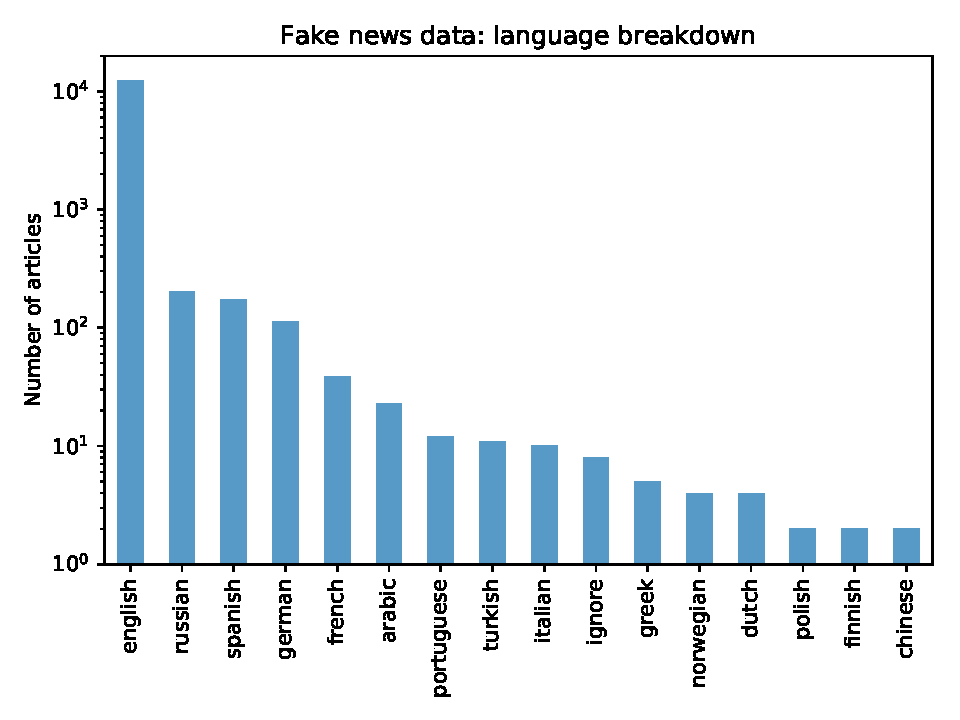
\includegraphics[scale=0.8]{plots/fake_languages}
\end{center}
\end{figure}

Since the algorithm is based on word frequency, it seems like a good idea
to discard all the non-English articles from the dataset ($\sim$2\% of the total),
as described also in Sec. \ref{sec:preproc}.

After this selection, the dataset consists of 34359 rows, 22002 real news articles and 12357 fake news articles.
The size of the dataset is about 120 MB. \\
Table \ref{tab:columns} summarises the columns of the dataset.
Most of them are not used in any stage of this project, but are kept for consistency.
For some columns the description is not provided,
because not known or not completely clear to the author.
Some of the variables are visualized in Sec. \ref{sec:visuals}.

\begin{table}
\footnotesize
\begin{center}
\begin{tabular}{ c | c | c | c }
\textbf{Name} & \textbf{Type} & \textbf{Description} & \textbf{Comments} \\ \hline
\texttt{author} & str & Author of the post & - \\ \hline
\texttt{comments} & int & Number of comments to the post & more in ``Exploratory Visualization'' \\ \hline
\texttt{country} & str & Country of the post & - \\ \hline
\texttt{crawled} & str & Date/time/timezone crawling information & - \\ \hline
\texttt{domain\_rank} & float & NA & - \\ \hline
\texttt{label} & int & 1 for fake, 0 for real & Output label \\ \hline
\texttt{language} & str & Language of the post & - \\ \hline
\texttt{likes} & int & Number of likes to the post & more in ``Exploratory Visualization'' \\ \hline
\texttt{main\_img\_url} & str & Url of the main image in the article & - \\ \hline
\texttt{ord\_in\_thread} & int & NA & - \\ \hline
\texttt{participants\_count} & int & Number of participants to the thread & more in ``Exploratory Visualization'' \\ \hline
\texttt{published} & str & Date/time/timezone crawling information & - \\ \hline
\texttt{replies\_count} & int & Number of replies to the post & more in ``Exploratory Visualization'' \\ \hline
\texttt{shares} & int & Number of shares & more in ``Exploratory Visualization'' \\ \hline
\texttt{site\_url} & str & Url of the website of the post & - \\ \hline
\texttt{spam\_score} & float & NA & - \\ \hline
\texttt{text} & str & Text of the news & Discriminating feature \\ \hline
\texttt{thread\_title} & str & NA & - \\ \hline
\texttt{title} & str & Title of the post & more in ``Exploratory Visualization'' \\ \hline
\texttt{uuid} & str & NA & - \\
\end{tabular}
\end{center}
\caption{Summary of the 20 columns present in the dataset. \label{tab:columns}}
\end{table}

\subsection{Exploratory Visualization}
\label{sec:visuals}
Even though only one feature in the dataset is actually used for discrimination
in the classification task, it's nonetheless interesting to visualise
some of the other columns in the dataset (see Tab. \ref{tab:columns}).
In doing so, the fake/real news are plotted separately to better understand
the different trends across the two classes. \\
In Fig. \ref{fig:text_title_length} the number of characters in
the text and title of the article are shown.
Two observations are worth mentioning:
\begin{itemize}
\item Many fake news have a short text. This is somehow expected,
as there are not many arguments to describe to support a made up story...
\item Fake news tend to have slightly longer titles.
One possible explanation for this feature is the average lower level
of professionalism among the writers of fake news: a professional
journalist, in fact, knows that titles should be short to be more effective.
\end{itemize}
In Fig. \ref{fig:post_feedback} the
number of participants to the thread, replies to the thread and likes are respectively shown.
The only striking difference is about the number of likes, which is
significantly larger, as one would expect, for real news compared to fake news. \\
Finally in Fig. \ref{fig:wcloud} two examples of ``word cloud'' plots are shown,
where the words in the document are arranged in order to enphasise
the most frequent ones. These plots are generated using the \texttt{wordcloud} package \cite{wordcloud}.

%\newpage
\begin{figure}[h!]
\caption{The number of characters in the article text (left) and title (right). \label{fig:text_title_length}}
\begin{center}
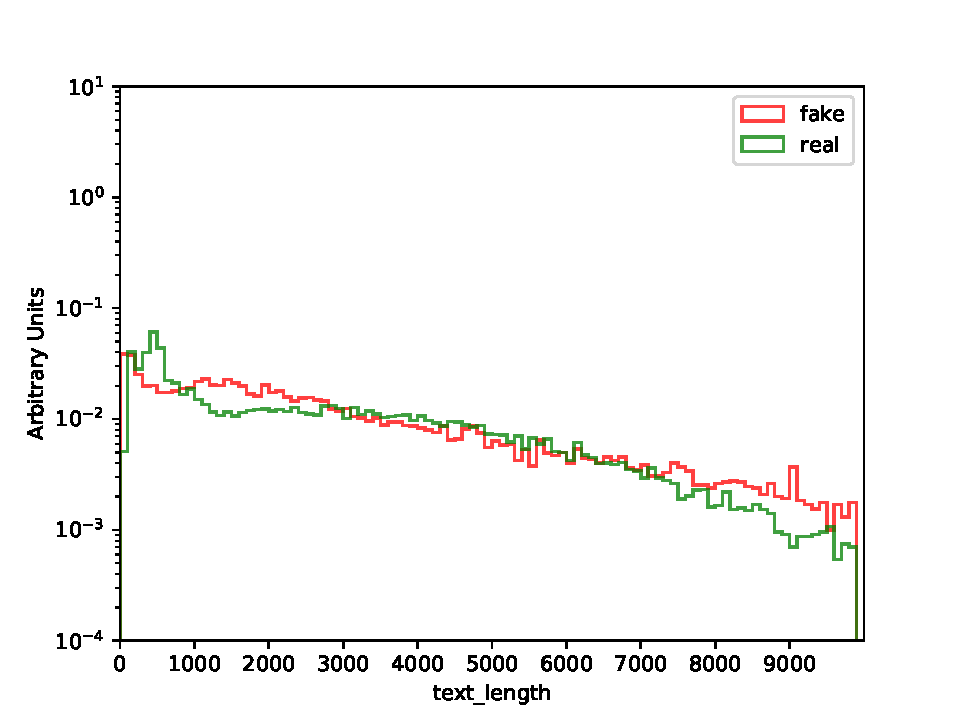
\includegraphics[width=0.4\textwidth]{plots/text_length} \hspace{0.2cm}
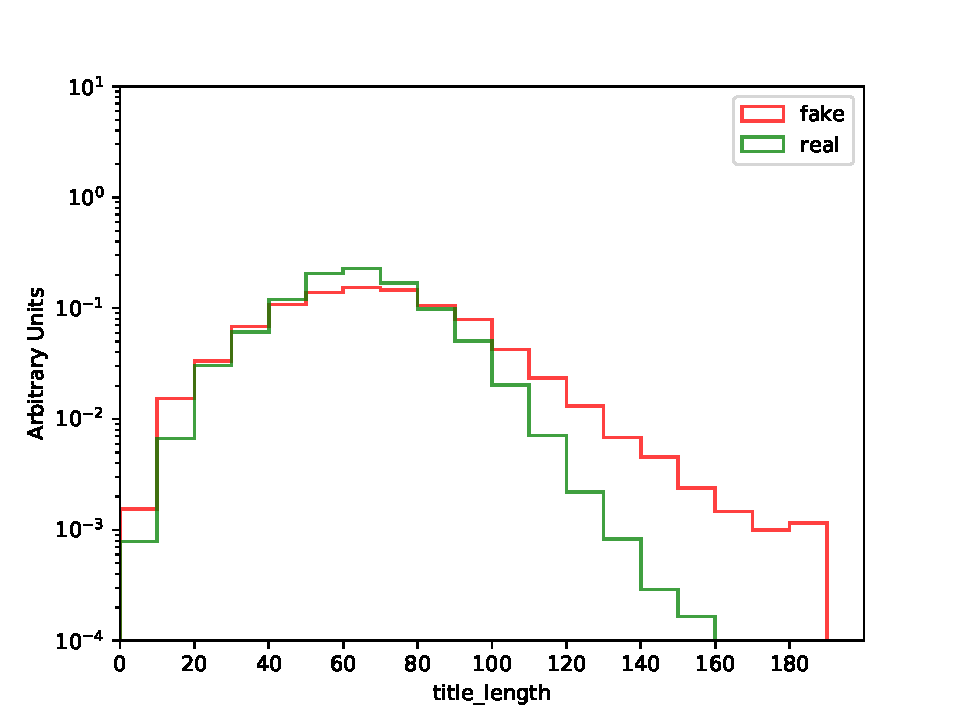
\includegraphics[width=0.4\textwidth]{plots/title_length}
\end{center}
\end{figure}

\begin{figure}[h!]
\caption{The number of participants in the thread (top left), replies to the thread (top right)
and likes to the post (bottom). \label{fig:post_feedback}}
\begin{center}
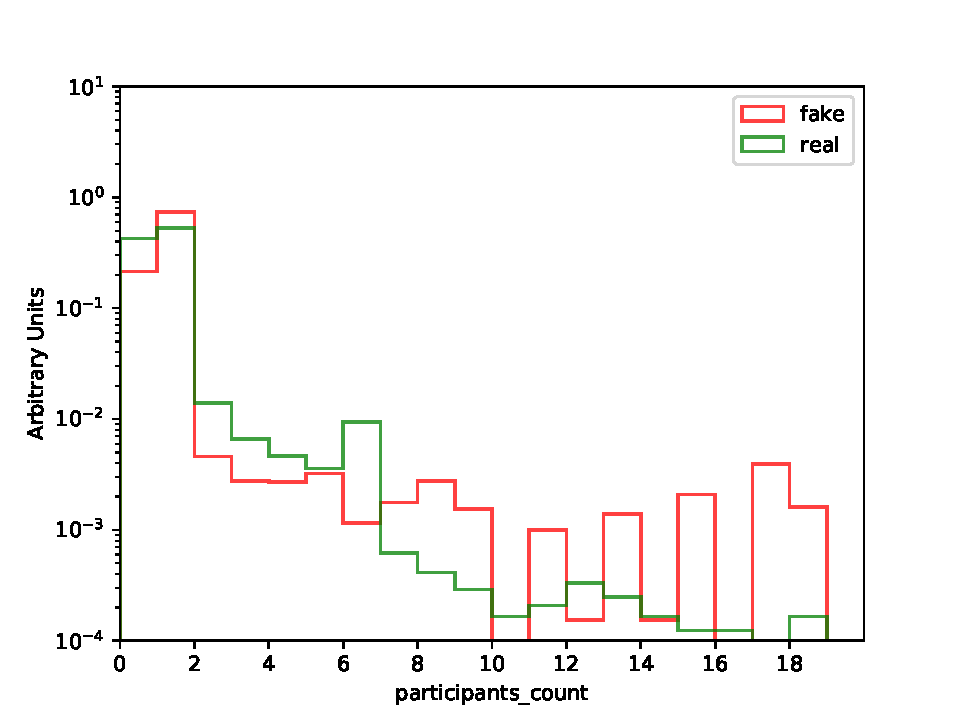
\includegraphics[width=0.4\textwidth]{plots/participants_count} \hspace{0.2cm}
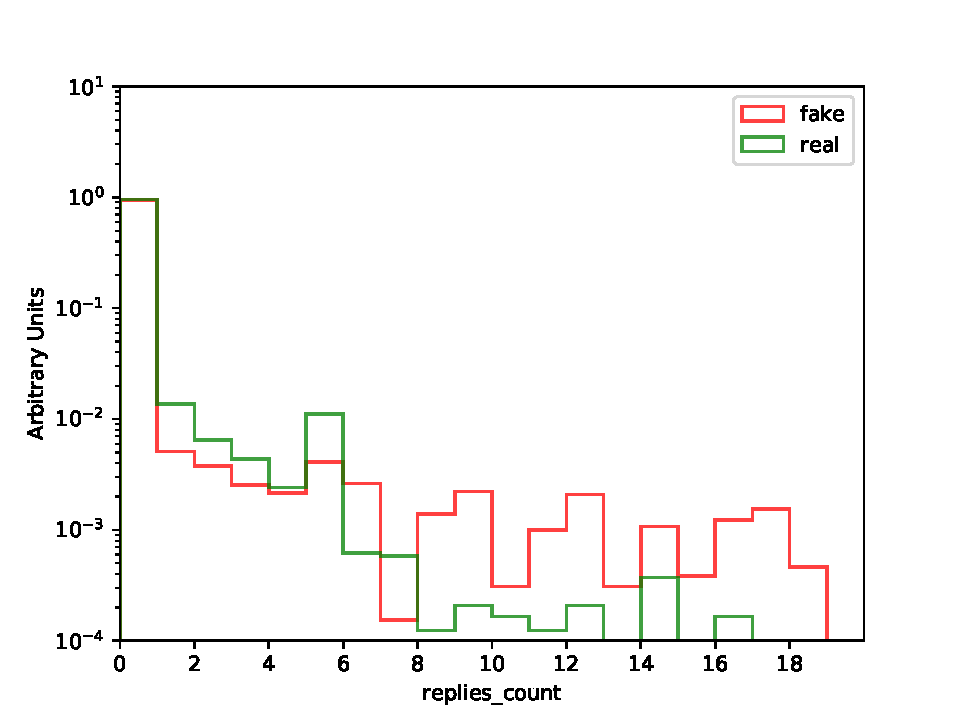
\includegraphics[width=0.4\textwidth]{plots/replies_count} \\
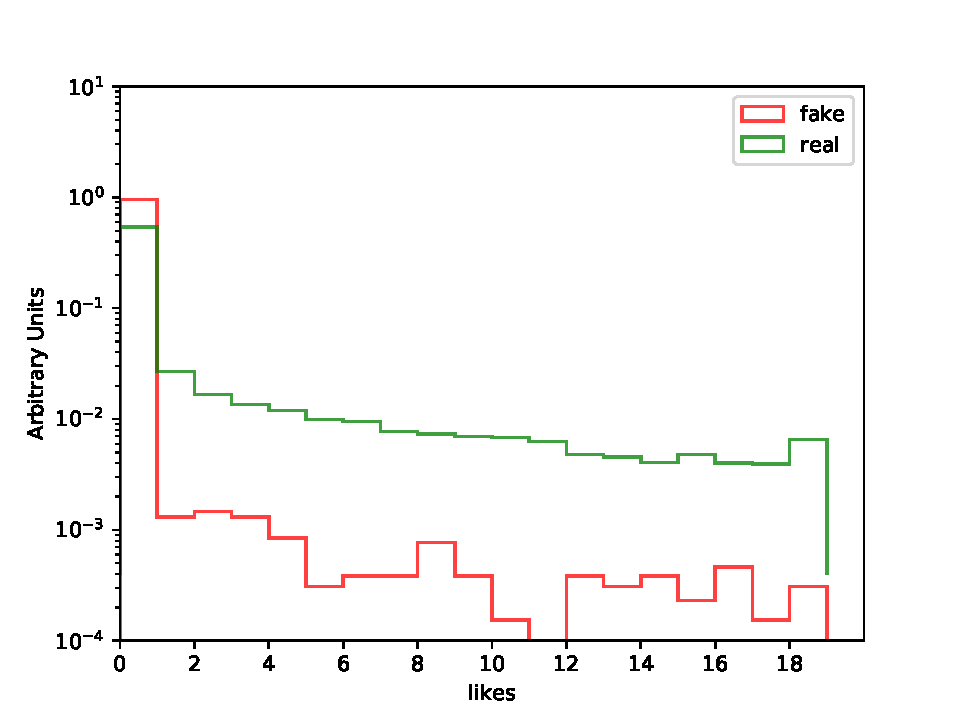
\includegraphics[width=0.4\textwidth]{plots/likes}
\end{center}
\end{figure}

\begin{figure}[h!]
\caption{Two examples of ``word cloud'' plots from a fake (left) and real (right) news. \label{fig:wcloud}}
\begin{center}
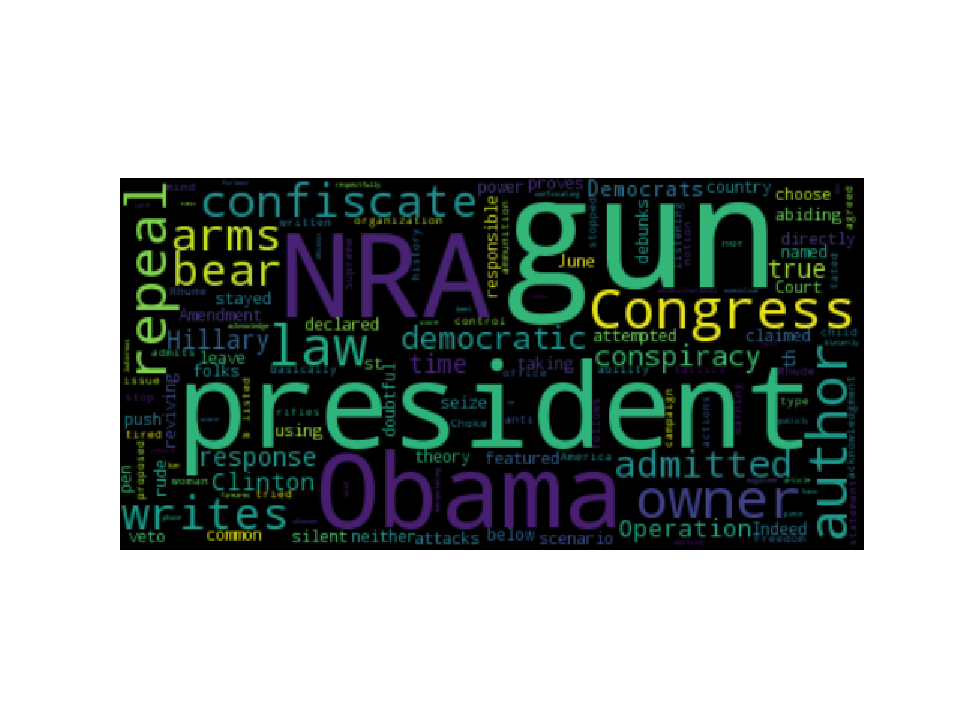
\includegraphics[width=0.4\textwidth]{plots/wcloud_fake} \hspace{0.2cm}
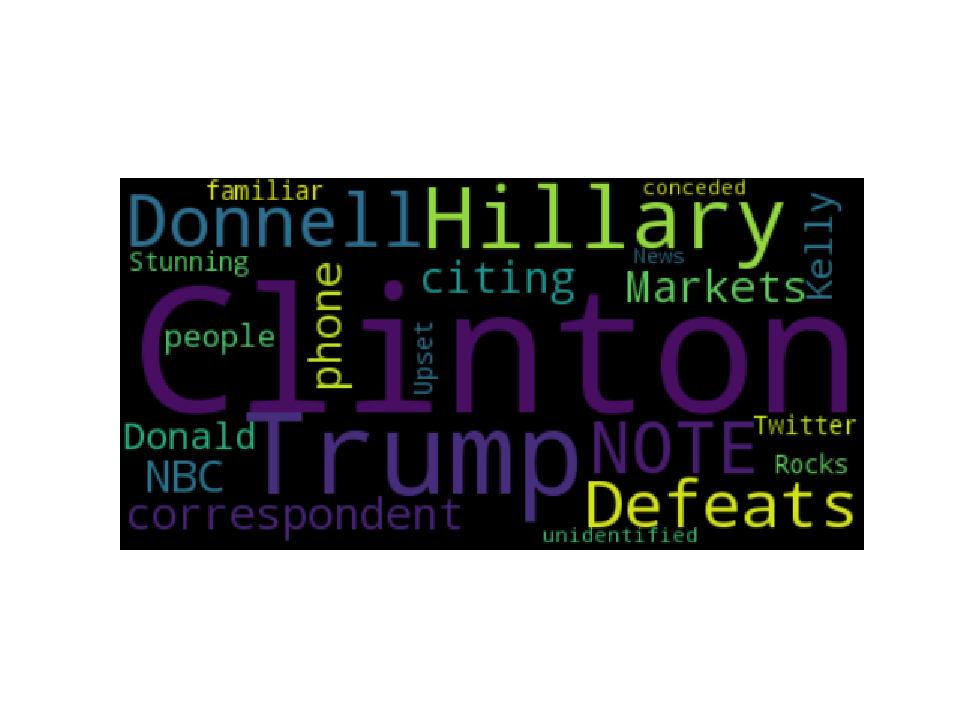
\includegraphics[width=0.4\textwidth]{plots/wcloud_real}
\end{center}
\end{figure}

\newpage
\subsection{Algorithms and Techniques}
\label{sec:algos}
As mentioned in Sec. \ref{sec:problem_statement}, several steps involving
different techniques are implemented, which will be thoroughly described in this section.

The very first transformation has to convert the text into numerical features,
as most of the ML algorithms work only with numerical inputs.
In this project we chose a popular technique called \textbf{Term Frequency-Inverse Document Frequency}
or simply \textbf{TFIDF} \cite{TFIDF}.
The TFIDF transformation allows not only to vectorize the text (i.e. the rows of the dataset)
into numerical features but naturally filters the most frequent words in the corpus,
as it is explained in the following. \\
The default \texttt{scikit-learn} implementation of TFIDF used in this project defines:
\begin{equation}
TFIDF (t, d) = TF(t, d) \times IDF (t)
\end{equation}
where the term frequency (TF) of term $t$ appearing $f_{t}$ times in document $d$ is defined as
\footnote{this definition of TF with the damping logarithm is referred to as \textit{sublinear TF} and
is meant to reduce the importance of terms with high frequency.}:
\begin{equation}
TF (t, d) = 1 + log(f_{t})
\end{equation}
and the inverse document frequency is defined as:
\begin{equation}
IDF (t) = log \frac{1+N}{1+n_{t}} + 1
\end{equation}
with $N$ being the total number of documents in the corpus and $n_{t}$ the number
of documents containing the term $t$.\\
After TFIDF is applied, the word vectors are normalized using the usual euclidean definition. \\
In order to reduce the number of features, the vocabulary is built discarding the
30\% of the most used terms in the corpus.

Another important ingredient is the ML algorithm to use for the classification.
We decided to test 3 different algorithms in order to cover different techniques with different assumptions
and training complexity.
\begin{itemize}
\item \textbf{Mulinomial Naive Bayes}. NB is frequently used in text classification,
like spam detection, because, despite its simplicity and ``naive'' assumptions (independence of features),
it proved to work still quite well in practice. It is also very fast to train.
\item \textbf{Logistic Regression Classifier}. Linear classifiers are usually a good compromise between
complexity and training time and therefore are a good benchmark to compare against more complicated algorithms.
\item \textbf{Random Forest}. Random forests are among the most powerful predictive
models and have a wide range of applications. The RF can potentially captures
more complex patterns in the dataset at the prize of a longer training and higher
parameter tuning complexity.
\end{itemize}
The three classifiers are finally combined in a ``voting classifier'' \cite{scikit-ensemble}.
The \textbf{ensemble classifier} usually gives better performances (smaller variance) compared to each single classifier in the
ensemble when there is little or none correlation across the different predictors
(different assumptions, different training set, etc.).

\subsection{Benchmark}
\label{sec:benchmark}
Some attempts have already been perfomed to detect fake news using ML algorithms \cite{Genes, NYDSA, jarmul}.
In these projects, typical F1 scores on the test set range from 80\% to 95\%.
Similar perfomances are expected also as a result of this project.

%----------------------------------------------------------------------------------------
%	METHODOLOGY SECTION
%----------------------------------------------------------------------------------------

\section{Methodology}


\subsection{Data Preprocessing}
\label{sec:preproc}
Since the real news dataset has only articles in English,
in the Kaggle dataset (fake news) only the articles
in English are retained (about 95\% of the total). \\
The real news dataset is huge and consists of about 500k news articles, in the
(quite inconvenient) format of a single json file per news.
We apply an additional processing on top of these corpus, which
consists of producing a single file and restricting the sources of news
to the following list: \textit{New York Times}, \textit{Washington Post},
\textit{The Washington Journal},
\textit{Reuters}, \textit{The Guardian}, \textit{Forbes},
\textit{BBC}, \textit{NPR} and \textit{Bloomberg}.
These websites are universally recognised as trustable sources of
information and we are confident that they represent an unbiased
sample of real news. \\
As the number of news remaining is still much larger
than the fake news ($\sim$100k vs. $\sim$13k), we further skim
by ``capping'' each source to a maximum of 3k articles,
chosen randomly. This procedure ensures that there is no source which
dominates the others, thus making the dataset more balanced (we
noticed that a sizeable fraction of news come from Reuters alone).
After this additional step we are left with about $\sim$24k articles.\\
A few articles have NAs in the \texttt{text} column and are also removed. \\
Finally, the labels are ``binarized'' as follows:
\begin{itemize}
\item \textbf{fake news} are assigned \texttt{label=1}
\item \textbf{real news} are assigned \texttt{label=0}
\end{itemize}

The dataset consists of 20 columns.
Only the \texttt{text} is used as discriminating feature in the
algorithm. However, the other variables are also used in the exploratory phase,
see Sec. \ref{sec:explore} and \ref{sec:visuals}.



\subsection{Implementation}
\label{sec:implementation}
The data is manipulated using \texttt{pandas} \cite{mckinney-proc-scipy-2010}.
The implementation of ML models and metrics relies on the \texttt{scikit-learn} API \cite{scikit-learn}.

Once the data is loaded, the first step is to divide it into \textit{training} and \textit{testing} datasets.
The common choice of retaining 20\% of the data for testing is adopted. \\
The article text is then transformed into numerical features according to the TFIDF procedure
described in Sec. \ref{sec:algos}. The \texttt{sklearn.feature\_extraction.text.TfidfVectorizer} \cite{scikit-tfidf}
class is used, with the following arguments:

\begin{lstlisting}[language=Python]
vectorizer = TfidfVectorizer(max_df=0.7,
                             stop_words='english')
\end{lstlisting}

\texttt{max\_df} is the fraction of words in the dictionary which are used as features:
in this implementation the 30\% most frequently used words will be discarded.
The \texttt{stopwords} option select the English list of ``stop-words'' implemented in the package.

Then the Multinomial Naive Bayes (MNB) classifier is defined \\
(class \texttt{sklearn.naive\_bayes.MultinomialNB} \cite{scikit-mnb})
using the default parameters and fitted to the training data.

The Logistic Regression (LRE) classifier is defined using the class \\
\texttt{sklearn.linear\_model.LogisticRegressionCV} \cite{scikit-lr}.
All the parameters of the constructor are the default ones.

For the implementation of the Random Forest (RFO) classifier the class\\
\texttt{sklearn.ensemble.RandomForestClassifier} \cite{scikit-rndf} is used.
Since there is a very large number of features and samples, the trees of the forest can
potentially grow very complicated. Hence, a high level of regularization is needed.
The first attempt of parameter set, which is tweaked afterwards using grid search, is as follows:
\begin{lstlisting}[language=Python]
clf_rndf = RandomForestClassifier(class_weight='balanced_subsample',
                                  n_estimators=30,
                                  max_depth=20,
                                  min_samples_split=20,
                                  max_features=0.01)
\end{lstlisting}
This choice is driven by the need to:
\begin{itemize}
    \item account for unbalance across classes (\texttt{class\_weight})
    \item reduce the number of input features (\texttt{max\_features})
    \item limit the size of the forest (\texttt{n\_estimators})
    \item regularize the trees (\texttt{max\_depth}, \texttt{min\_samples\_split})
\end{itemize}


The metrics described in Sec. \ref{sec:metrics} are computed using the
implementation in the \texttt{sklearn.metrics} module \cite{scikit-metrics}.


\subsection{Refinement}
\label{sec:refinement}
This section describes how the models implemented as of Sec. \ref{sec:implementation} are
fine-tuned and how the ensemble of classifier is defined.

The tuning of the hyperparameters is done using the powerful\\
\texttt{sklearn.model\_selection.GridSearchCV} class \cite{scikit-gridsearchcv}.
The hyper-parameters in the grids and their best fit values are reported in Tab. \ref{tab:bestfit}.

\begin{table}
\begin{center}
\begin{tabular}{ c | c | c }
\textbf{Model} & \textbf{Parameter} & \textbf{Best fit value} \\ \hline
\multirow{2}{*}{MNB} & \texttt{alpha} & 0.2 \\
 & \texttt{fit\_prior} & False \\ \hline
\multirow{4}{*}{LRE} & \texttt{C} & 20.4 \\
 & \texttt{dual} & True\\
 & \texttt{fit\_intercept} & True\\
 & \texttt{penalty} & 'l2'\\ \hline
\multirow{4}{*}{RFO} & \texttt{n\_estimators} & 100 \\
 & \texttt{max\_features} & 0.02 \\
 & \texttt{max\_depth} & 100 \\
 & \texttt{min\_samples\_split} & 50 \\ \hline
\end{tabular}
\end{center}
\caption{Best fit values of the floating parameters in the models.
\label{tab:bestfit}}
\end{table}

Two approaches for the ensemble are considered:
\begin{itemize}
\item Ensemble 1 (EN1): ``hard'' voting, i.e. majority voting, including all the 3 classifiers.
\item Ensemble 2 (EN2): ``soft'' voting, i.e. voting weighted by probabilities, including the LRE and RFO classifiers.
In this case the MNB is excluded because the probabilities computed by naive bayes
algorithms are known to be not trustable.
\end{itemize}

All the solutions and their performances are presented in Tab. \ref{tab:results}.
Based on these results, the chosen final model is EN2.

%----------------------------------------------------------------------------------------
%	RESULTS SECTION
%----------------------------------------------------------------------------------------

\section{Results}

\subsection{Model Evaluation and Validation}
All the results for intermediate and final solutions, based on the test set,
are presented in Tab. \ref{tab:results}.
It can be noticed that the optimisation improved largely the results
of the MNB model and the RFO model.
The LRE model instead is not improved significantly. \\
The EN2 has slightly better perfomances, with F1-score of 92\% and
it's chosen as the final model. \\
Overall the performances are very good and satisfactory also
compared to the benchmarks reported in Sec. \ref{sec:benchmark}.

\begin{table}
\begin{center}
\begin{tabular}{ c | c | c | c | c }
\textbf{Classifier} & \textbf{Accuracy} & \textbf{Precision} & \textbf{Recall} & \textbf{F1 score} \\ \hline
\multicolumn{5}{c}{\textbf{before optimisation}} \\ \hline
MNB & 0.84 & 0.56 & 0.97 & 0.71 \\ \hline
LRE & 0.94 & 0.93 & 0.91 & 0.92 \\ \hline
RFO & 0.88 & 0.91 & 0.79 & 0.85 \\ \hline
\multicolumn{5}{c}{\textbf{after optimisation}} \\ \hline
MNB & 0.90 & 0.87 & 0.86 & 0.86 \\ \hline
LRE & 0.94 & 0.93 & 0.91 & 0.92 \\ \hline
RFO & 0.93 & 0.89 & 0.91 & 0.90 \\ \hline
\multicolumn{5}{c}{\textbf{ensembles}} \\ \hline
EN1 & 0.94 & 0.92 & 0.91 & 0.92 \\ \hline
{\color{red} EN2} & {\color{red} 0.95} & {\color{red} 0.92} & {\color{red} 0.92} & {\color{red} 0.92} \\ \hline
\end{tabular}
\end{center}
\caption{Performances of the 3 classifiers (before and after optimization)
and the 2 ensemble classifiers (in red the final model).
\label{tab:results}}
\end{table}

To further assess the validity of the model, an additional \textit{sensitivity test} is carried out:
in each article of the dataset one sentence is removed, chosen randomly.
The results prove to be stable against this check: in particular the F1-score
is still 92\% even after this perturbation.


\subsection{Justification}
The final model is a soft-voting ensemble classifier which
consists of a Logistic Regression model combined with a Random Forest model,
both highly regularized.
The final solution has an F1-score of 92\% on the test set,
with perfectly balanced recall and sensitivity. These performances are
in line with the ones reported in the benchmarks \cite{NYDSA, jarmul}.

Despite the good results obtained with this dataset,
we can't claim that the problem of fake news is solved by this algorithm.
There are in fact limitations to its use that are further discussed
in Sec. \ref{sec:improvement}.


%----------------------------------------------------------------------------------------
%	CONCLUSION SECTION
%----------------------------------------------------------------------------------------

\section{Conclusion}

\subsection{Free-form visualization}
One of the most important characteristics of ML models is the number
of samples needed for training.
In fact, everytime the model has to be re-trained on new data, it's crucial to know
the number of samples in the training set which is needed to achieve optimal perfomances.
In Fig. \ref{fig:scores_vs_nsamples} several different scores are shown as a function
of the number of samples included in the training dataset, namely accuracy, precision, recall and F1-score
(see Sec. \ref{sec:metrics}).
In this analysis the test set is the same for each training session.
\begin{figure}[h!]
\caption{Classification scores as a function of the number of training samples. \label{fig:scores_vs_nsamples}}
\begin{center}
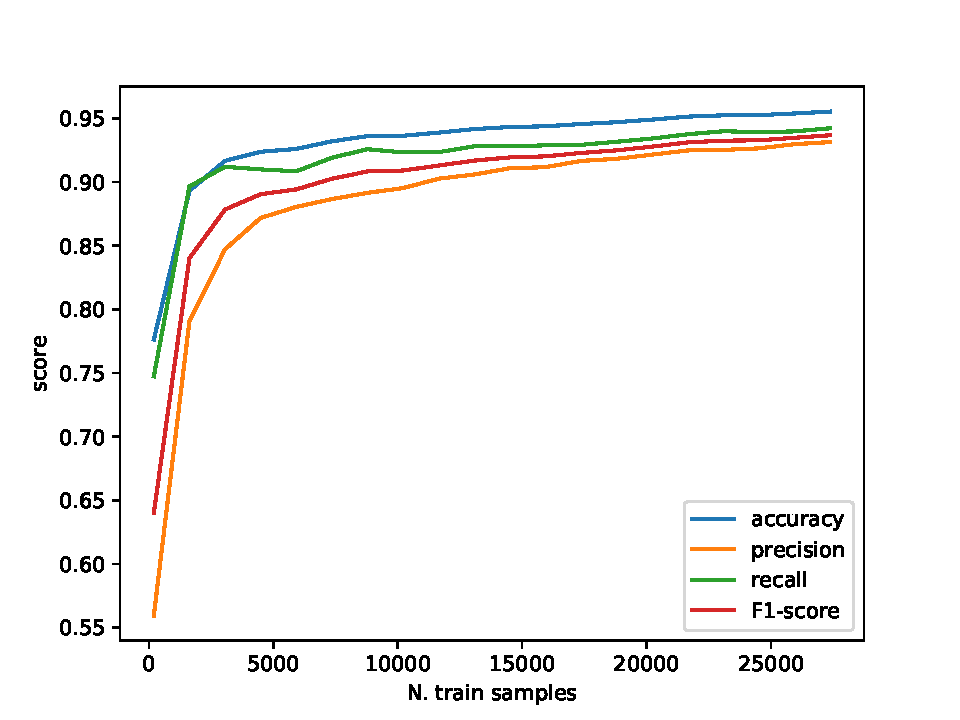
\includegraphics[scale=0.8]{plots/scores_vs_nsamples.pdf}
\end{center}
\end{figure}
Looking in particular at the F1-score, which is the main metric used in the project,
the following observations can be made:
\begin{itemize}
    \item with the available size of training dataset there seems to be no complete ``saturation'' of performances,
    as the scores don't seem to reach a flat ``plateau''.
    However, the increase in performances is very slow above about 10000 training samples.
    \item on the other hand, the number of training samples needed to achieve good perfomances is quite small:
    with about 1500 samples the F1-score is already 85\%.
\end{itemize}

\subsection{Reflection}
\label{sec:reflection}
In this project the problem of detecting the so-called ``fake news'' has been studied.
A ML algorithm has been developed which by analyzing the text of the article
returns the result of the binary classification: fake news/real news. \\
First, a suitable dataset of fake news and real news have been identified and downloaded.
Then the article text in each instance has been converted to a vector of numerical features,
representing a set of weights which take into account the frequency of the word in the document and
in the corpus (TFIDF vectorization).
The resulting ``word vectors'' have been feeded to 3 different ML models which are
compared using the appropriate metrics.
An ensemble including the best 2 classifiers is used as final model.

There are several interesting aspects of this project.
In particular the following points have been very stimulating challenges to solve.

\begin{itemize}
\item \textbf{Find the datasets} \\
    While the idea for this project came when we stumbled upon the Kaggle fake news dataset,
    the real news dataset has been more difficult to collect.
    Several news website do not provide an API to fetch historical articles and most
    of them don't provide the access to the full article.
    Only after quite some research, we found the webhose.io dataset which fit all these criteria.
\item \textbf{Feature extraction} \\
    Being the first project of ``text analysis'' that I carry out,
    I was lacking some knowledge about how to transform the text into features.
    It took me some time to go through the different options (\textit{bag-of-words},
    \textit{word2vec}, \textit{TFIDF}) and understand which one was the best for this case.
\item \textbf{Model regularization} \\
    The regularization of the random forest model has been very challenging.
    In fact, in text analysis the number of features grows very large and a high
    level of regularization is needed for complicated models.
    With long training time and different combinations of parameters to validate,
    it took quite some effort to achieve an optimal solution.

\end{itemize}

\subsection{Improvement}
\label{sec:improvement}
There is room for improvement both in the model itself and in its validation.
Some ideas are described below: their implementation is, however, outside
the scope of this project.

Possible improvements on the algorithm side are:
\begin{itemize}
    \item use different, more ``complex'' models, like \textbf{deep neural networks};
    \item analyze \textbf{n-grams}, i.e. ensemble of $n$ words;
    \item incorporate also the \textbf{headline} of the article, together with the text;
\end{itemize}

On the validation side, the main limitation is that training/testing data belong to approximately the same time frame.
It should be checked how the performaces change when this assumptions is relaxed.
If the perfomances degrade, one should make sure that the model is trained on data that is relevant to
the new instances that are being classified.
This is not simple to handle from the technical point of view:
one has to fetch much more data than what has been used in this project and
probably needs to build a set of pre-trained models which cover a relevant time range.

%----------------------------------------------------------------------------------------
%	REFERENCES SECTION
%----------------------------------------------------------------------------------------

\nocite{*}
\bibliographystyle{ieeetr}
%\bibliographystyle{alphadin}
\renewcommand{\refname}{References}
\bibliography{references}

\end{document}
